\documentclass[xcolor=x11names,compress,professionalfonts]{beamer}

%% General packages %%%%%%%%%%%%%%%%%%%%%%%%%%%%%%%%%%
\usepackage[utf8]{inputenc}
\usepackage{graphicx}
\usepackage{tikz}
\tikzset{% change default arrow tips
    >=latex
}
\usepackage{ifthen}

\usepackage{amsmath}
\usepackage{nicefrac}

\usepackage{color}

%%%%%%%%%%%%%%%%%%%%%%%%%%%%%%%%%%%%%%%%%%%%%%%%%%%%%%


%% Beamer Layout %%%%%%%%%%%%%%%%%%%%%%%%%%%%%%%%%%
\useoutertheme[subsection=false,shadow]{miniframes}
\useinnertheme{rectangles}

\setbeamertemplate{navigation symbols}{}%remove navigation symbols

\newcommand{\btVFill}{\vskip0pt plus 1filll}%place an element at the bottom of the page

\usepackage{libertine}
\usepackage[T1]{fontenc}

\setbeamerfont{title like}{shape=\scshape}
\setbeamerfont{frametitle}{shape=\scshape}

\setbeamercolor*{lower separation line head}{bg=DeepSkyBlue4} 
\setbeamercolor*{normal text}{fg=black,bg=white} 
\setbeamercolor*{alerted text}{fg=red} 
\setbeamercolor*{example text}{fg=black} 
\setbeamercolor*{structure}{fg=black} 
 
\setbeamercolor*{palette tertiary}{fg=black,bg=black!10} 
\setbeamercolor*{palette quaternary}{fg=black,bg=black!10} 

\renewcommand{\(}{\begin{columns}}
\renewcommand{\)}{\end{columns}}
\newcommand{\<}[1]{\begin{column}{#1}}
\renewcommand{\>}{\end{column}}

\definecolor{BostonBlue}{HTML}{00688B}
\definecolor{Complementary}{HTML}{8B2300}
%%%%%%%%%%%%%%%%%%%%%%%%%%%%%%%%%%%%%%%%%%%%%%%%%%

\usepackage{braket}
% compile child documents using this preamble
\usepackage{subfiles}

%%%My Math

\newcommand{\pd}[2]{\frac{\displaystyle \partial #1}{\displaystyle\partial #2}} % for partial derivatives
\renewcommand{\d}[1]{\mathrm{d}#1}

\begin{document}

\begin{frame}
\title{Multifractality of the tight-binding eigenstates on the Fibonacci chain}

\author{ Nicolas Macé, Anuradha Jagannathan, Frédéric Piéchon}

\institute % (optional)
{
  Laboratoire de Physique des Solides\\
  Université Paris-Sud
}

\date{November 25, 2015}

\titlepage

\btVFill
\begin{columns}
\begin{column}{2cm}
~\\
~\\
~\\
~\\
\raggedright

\includegraphics[scale=.15]{LogoUPSUD.png}
\end{column}
\begin{column}{6cm}
\centering
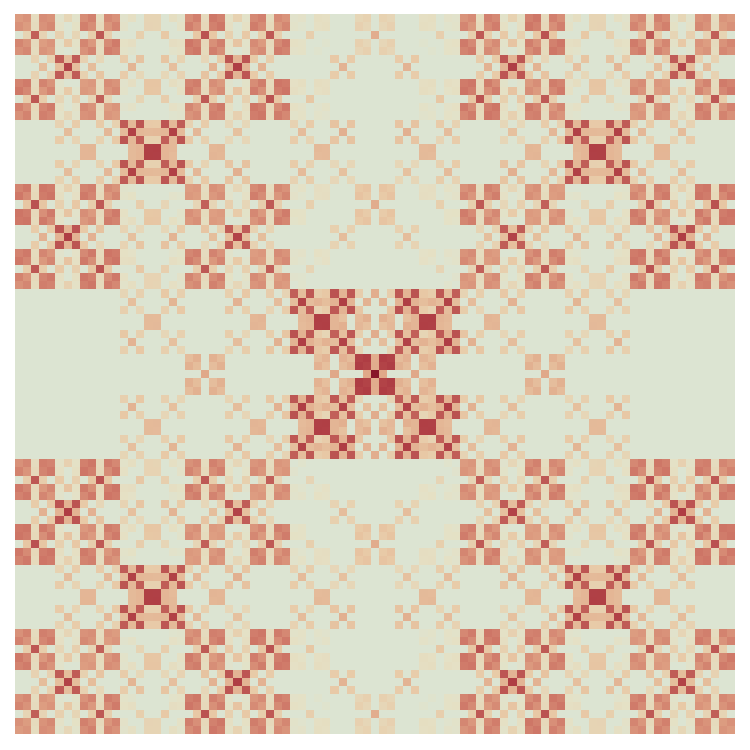
\includegraphics[width=.5\textwidth]{illustration.pdf}
\end{column}
\begin{column}{2cm}
~\\
~\\
~\\
~\\
\raggedleft

\includegraphics[scale=.15]{logo-lps.jpg}
\end{column}
\end{columns}
\end{frame}

\end{document}